%
% File naaclhlt2016.tex
%

\documentclass[11pt,letterpaper]{article}
\usepackage{style/naaclhlt2016}
\usepackage{times}
\usepackage{bbm}
\usepackage[usenames,dvipsnames]{color}
\usepackage[utf8]{inputenc}

\newif\ifcomment\commenttrue
% Preamble file contains handy macros and most packages you might want to use.
% At the start are packages that conflict with various styles.  Don't add them
% in!  Just put it in your main TeX file instead.

% Do not put either of these (subfigure or subfloat) into the preamble
% - they clash.  Use them in the final LaTeX document
% \usepackage{subfigure}
% \suepackage{subfloat}

% Do not use times in the preamble!  It just causes problems with some
% publication chairs (e.g., ICML 2013).  If you want it, put it in your own
% document.
% \usepackage{times}


% Breaks ACM-SIG style
% \usepackage{titlesec}
% \usepackage{amsthm}
% \usepackage{nomencl}

% comment out the following line, as it conflicts with aistats2012.sty
%\usepackage{caption}


% Below should be safe
\usepackage{framed}
\usepackage{mdwlist}
\usepackage{latexsym}
\usepackage{xcolor}
\usepackage{nicefrac}
\usepackage{booktabs}
\usepackage{amsfonts}
\usepackage{bold-extra}
\usepackage{amsmath}
\usepackage{dsfont}
\usepackage{amssymb}
\usepackage{bm}
\usepackage{graphicx}
\usepackage{mathtools}
\usepackage{microtype}
\usepackage{multirow}
\usepackage{multicol}
%\usepackage{url}
\usepackage{latexsym,comment}

\newcommand{\breakalign}{\right. \nonumber \\ & \left. \hspace{2cm}}



\newcommand{\feat}[1]{{\small \texttt{#1}}}
\newcommand{\act}[1]{{\small \texttt{#1}}}
\newcommand{\ngram}[0]{$n$-gram}
\newcommand{\topic}[1]{\underline{#1}}
\newcommand{\gem}[1]{\mbox{\textsc{gem}}}
\newcommand{\abr}[1]{\textsc{#1}}
\newcommand{\camelabr}[2]{{\small #1}{\textsc{#2}}}
\newcommand{\abrcamel}[2]{{\textsc #1}{\small{#2}}}
\newcommand{\grammar}[1]{{\color{red} #1}}
\newcommand{\explain}[2]{\underbrace{#2}_{\mbox{\footnotesize{#1}}}}
\newcommand{\dir}[1]{\mbox{Dir}(#1)}
\newcommand{\bet}[1]{\mbox{Beta}(#1)}
\newcommand{\py}[1]{\mbox{\textsc{py}}(#1)}
\newcommand{\td}[2]{\mbox{\textsc{TreeDist}}_{#1} \left( #2 \right)}
\newcommand{\yield}[1]{\mbox{\textsc{Yield}} \left( #1 \right)}
\newcommand{\mult}[1]{\mbox{Mult}( #1)}
\newcommand{\wn}{\textsc{WordNet}}
\newcommand{\twentynews}{\textsc{20news}}
\newcommand{\g}{\, | \,}
\newcommand{\Gam}[1]{\Gamma \left( \textstyle #1 \right)}
\newcommand{\LG}[1]{\log \Gamma \left( \textstyle #1 \right)}
\newcommand{\Pois}[1]{\mbox{Poisson}(#1)}
\newcommand{\pcfg}[3]{#1_{#2 \rightarrow #3}}
\newcommand{\grule}[2]{#1 \rightarrow #2}
\newcommand{\kl}[2]{D_{\mbox{\textsc{KL}}} \left( #1 \,||\, #2 \right)}

\newcommand{\digambig}[1]{\Psi \left( #1 \right) }
\newcommand{\digam}[1]{\Psi \left( \textstyle #1 \right) }
\newcommand{\ddigam}[1]{\Psi' \left( \textstyle #1 \right) }

\DeclareMathOperator*{\argmax}{arg\,max}
\DeclareMathOperator*{\argmin}{arg\,min}
\newcommand{\bmat}[1]{\text{\textbf{#1}}}
\newcommand{\bvec}[1]{\boldsymbol{#1}}

\newcommand{\email}[1]{ {\small \href{mailto://#1}{\texttt{#1} }  }}
\newcommand{\emaillink}[2]{ {\small \href{mailto://#2}{\texttt{#1} }  }}

\newcommand{\ch}[1]{\begin{CJK*}{UTF8}{gbsn}#1\end{CJK*}}

\newcommand{\e}[2]{\mathbb{E}_{#1}\left[ #2 \right] }
\newcommand{\h}[2]{\mathbb{H}_{#1}\left[ #2 \right] }
\newcommand{\ind}[1]{\mathds{1}\left[ #1 \right] }
\newcommand{\ex}[1]{\mbox{exp}\left\{ #1\right\} }
\newcommand{\D}[2]{\frac{\partial #1}{\partial #2}}
\newcommand{\elbo}{\mathcal{L}}

\newcommand{\hidetext}[1]{}
\newcommand{\ignore}[1]{}

\newcommand{\todo}[1]{\textcolor{red}{{\bf TODO: #1}}}

\ifcomment
\newcommand{\pinaforecomment}[3]{\colorbox{#1}{\parbox{.8\linewidth}{#2: #3}}}
\else
\newcommand{\pinaforecomment}[3]{}
\fi

\newcommand{\jbgcomment}[1]{\pinaforecomment{red}{JBG}{#1}}
\newcommand{\mjpcomment}[1]{\pinaforecomment{blue}{MJP}{#1}}
\newcommand{\czcomment}[1]{\pinaforecomment{orange}{chen}{#1}}
\newcommand{\ffcomment}[1]{\pinaforecomment{red}{FF}{#1}}
\newcommand{\fpcomment}[1]{\pinaforecomment{green}{FP}{#1}}
\newcommand{\yhcomment}[1]{\pinaforecomment{green}{YH}{#1}}
\newcommand{\hhecomment}[1]{\pinaforecomment{blue}{HH}{#1}}
\newcommand{\tncomment}[1]{\pinaforecomment{blue}{TN}{#1}}
\newcommand{\mnicomment}[1]{\pinaforecomment{green}{Mohit}{#1}}
\newcommand{\prcomment}[1]{\pinaforecomment{lightblue}{Pedro}{#1}}
\newcommand{\fscomment}[1]{\pinaforecomment{orange}{Shi}{#1}}
\newcommand{\vmcomment}[1]{\pinaforecomment{yellow}{Varun}{#1}}
\newcommand{\rscomment}[1]{\pinaforecomment{yellow}{Richard}{#1}}
\newcommand{\jszcomment}[1]{\pinaforecomment{green}{JSG}{#1}}
\newcommand{\ascomment}[1]{\pinaforecomment{blue}{AS}{#1}}
\newcommand{\vecomment}[1]{\pinaforecomment{blue}{VE}{#1}}
\newcommand{\halcomment}[1]{\pinaforecomment{magenta!20}{Hal}{#1}}
\newcommand{\kgcomment}[1]{\pinaforecomment{blue}{Kim}{#1}}
\newcommand{\vancomment}[1]{\pinaforecomment{green}{VAN}{#1}}
\newcommand{\thangcomment}[1]{\pinaforecomment{green}{Thang}{#1}}
\newcommand{\alvincomment}[1]{\pinaforecomment{cyan}{Alvin}{#1}}
\newcommand{\reviewercomment}[1]{\pinaforecomment{blue}{Reviewer}{#1}}
\newcommand{\brscomment}[1]{\pinaforecomment{blue}{BRS}{#1}}
\newcommand{\psrcomment}[1]{\pinaforecomment{yellow}{PSR}{#1}}
\newcommand{\zkcomment}[1]{\pinaforecomment{cyan}{ZK}{#1}}
\newcommand{\swcomment}[1]{\pinaforecomment{yellow}{SW}{#1}}
\newcommand{\shaycomment}[1]{\pinaforecomment{yellow}{SBC}{#1}}
\newcommand{\jlundcomment}[1]{\pinaforecomment{cyan}{J}{#1}}
\newcommand{\kdscomment}[1]{\pinaforecomment{ceil}{KDS}{#1}}
\newcommand{\lkfcomment}[1]{\pinaforecomment{yellow}{LF}{#1}}
\newcommand{\yfcomment}[1]{\pinaforecomment{brown}{YF}{#1}}
\newcommand{\ewcomment}[1]{\pinaforecomment{lightblue}{Eric}{#1}}

\newcommand{\smalltt}[1]{ {\tt \small #1 }}
\newcommand{\smallurl}[1]{ \begin{tiny}\url{#1}\end{tiny}}
%\newcommand{\smallurl}[1]{ \begin{tiny} HIDDEN \end{tiny}}
\newenvironment{compactenum}{ \begin{enumerate*} \small }{ \end{enumerate*} }

\definecolor{lightblue}{HTML}{3cc7ea}
\definecolor{CUgold}{HTML}{CFB87C}
\definecolor{grey}{rgb}{0.95,0.95,0.95}
\definecolor{ceil}{rgb}{0.57, 0.63, 0.81}


% Datasets

\newcommand{\qb}[0]{Quizbowl}
\newcommand{\triviaqa}{\camelabr{Trivia}{qa}}
\newcommand{\qblink}{\abrcamel{qb}{Link}}
\newcommand{\qanta}{\textsc{qanta}}


\makeatletter
\newcommand{\@BIBLABEL}{\@emptybiblabel}
\newcommand{\@emptybiblabel}[1]{}
\makeatother
\usepackage{hyperref}

\naaclfinalcopy % Uncomment this line for the final submission
\def\naaclpaperid{490} %  Enter the naacl Paper ID here

% To expand the titlebox for more authors, uncomment
% below and set accordingly.
% \addtolength\titlebox{.5in}

\newcommand\BibTeX{B{\sc ib}\TeX}
\newcommand{\rmn}[0]{{\bf \textsc{rmn}}}
\newcommand{\grmn}[0]{{\bf \textsc{grmn}}}
\newcommand{\htmm}[0]{{\bf \textsc{htmm}}}
\newcommand{\lda}[0]{{\bf \textsc{lda}}}
\newcommand{\nubbi}[0]{{\bf \textsc{nubbi}}}
\newcommand{\norm}[1]{| #1 |}
\newcommand{\euclidean}[1]{\left\lVert #1 \right\rVert}
\newcommand{\rnn}[0]{{\bf \textsc{rnn}}}
\newcommand{\gru}[0]{{\bf \textsc{gru}}}
\newcommand{\bmat}[1]{\text{\textbf{#1}}}
\newcommand{\bvec}[1]{\boldsymbol{#1}}

\title{Feuding Families and Former Friends:\\Unsupervised Learning for Dynamic Fictional Relationships}

\author{
  Mohit Iyyer,$^{1}$ Anupam Guha,$^{1}$ Snigdha Chaturvedi,$^{1}$ Jordan Boyd-Graber,$^{2}$ Hal Daumé III$^{1}$\\
  $^1$University of Maryland, Department of Computer Science and \abr{umiacs}\\
        $^2$University of Colorado, Department of Computer Science \\
  {\tt \{miyyer,aguha,snigdac,hal\}@umiacs.umd.edu}, \\
  {\tt Jordan.Boyd.Graber@colorado.edu} \\
}

\begin{document}

\maketitle

\begin{abstract}
  Understanding how a fictional relationship between two characters changes over
  time (e.g., from best friends to sworn enemies) is a key challenge in digital
  humanities scholarship.  We present a novel unsupervised neural network for
  this task that incorporates dictionary learning to generate interpretable,
  accurate relationship trajectories. While previous work on characterizing
  literary relationships relies on plot summaries annotated with predefined
  labels, our model jointly learns a set of global relationship descriptors as
  well as a trajectory over these descriptors for each relationship in a dataset
  of raw text from novels. We find that our model learns descriptors of events
  (e.g., marriage or murder) as well as interpersonal states (love,
  sadness). Our model outperforms topic model baselines on two crowdsourced
  tasks, and we also find interesting correlations to annotations in an existing
  dataset.
\end{abstract}

\section{Describing Character Relationships}
\label{sec:introduction}

\begin{figure}[t!]
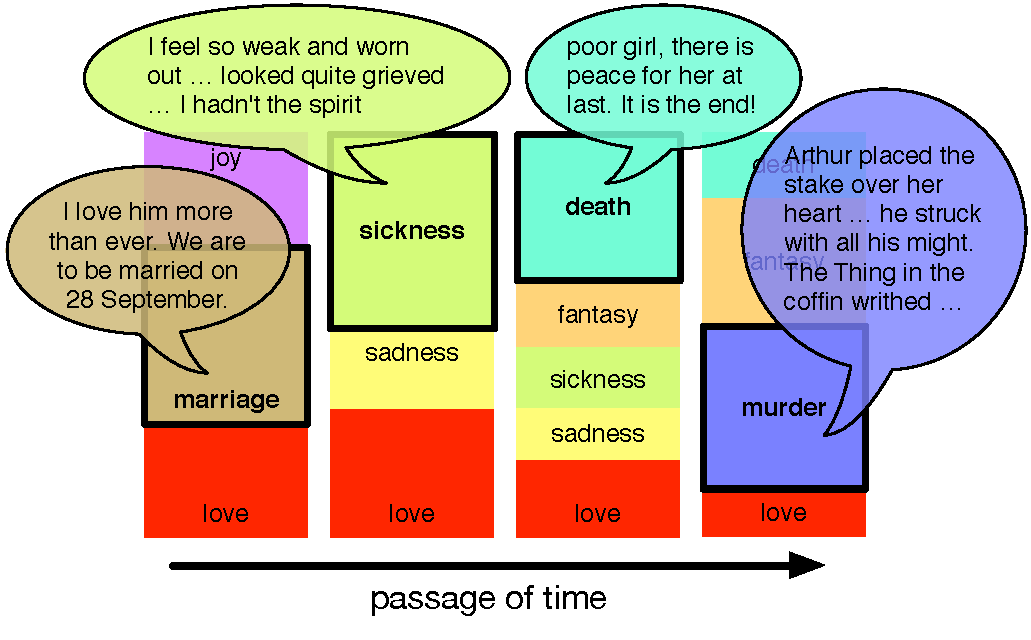
\includegraphics[width=1.0\linewidth]{2016_naacl_relationships/figures/lucy_and_arthur.pdf}
\caption{An example trajectory depicting the dynamic relationship between Lucy
  and Arthur in Bram Stoker's \textit{Dracula}, which starts with love and ends
  with Arthur killing the vampiric Lucy. Each column describes the relationship
  state at a particular time by weights over a set of descriptors (larger
  weights shown as bigger boxes). Our goal is to learn---without
  supervision---both the descriptors and the trajectories from raw fictional
  texts.}
\label{fig:traj}
\end{figure}

When two characters in a book break bread, is their meal just a result
of biological needs or does it mean more?
\newcite{goldthwaite-14} argue that this simple interaction reflects
the diversity and background of the characters, while
\newcite{foster-09} suggests that the tone of a meal can portend
either good or ill for the rest of the book. To support such theories,
scholars use their literary expertise to draw connections
between disparate books: Gabriel Conroy's dissonance from his family
at a sumptuous feast in Joyce's \emph{The Dead}, the frustration of
Tyler's mother in \emph{Dinner at the Homesick Restaurant}, and the
grudging respect for a blind man eating meatloaf in Carver's
\emph{Cathedral}.




However, these insights do not come cheap.  It takes years of careful
reading and internalization to make connections across
books, which means that relationship symmetries and archetypes are
likely to remain hidden in the millions of books published every year
unless literary scholars are actively searching for them.

Natural language processing techniques have been increasingly used to
assist in these literary investigations by discovering patterns in
texts~\cite{jockers-13}.  In Section~\ref{sec:related} we review
existing techniques that classify or cluster relationships between
characters in books using a fixed set of labels (e.g., friend or
enemy).  However, such approaches ignore interactions between
characters that lie outside of the established lexicon and cannot
account for the dynamic nature of relationships that evolve through
the course of a book, such as the vampiric downfall of Lucy and
Arthur's engagement in \textit{Dracula} (Figure~\ref{fig:traj}) or Winston Smith's
rat-induced betrayal of Julia in \textit{1984}.

To address these issues, we propose the task of unsupervised
relationship modeling, in which a model jointly learns a set of
\emph{relationship descriptors} as well as \emph{relationship
  trajectories} for pairs of literary characters. Instead of assigning
a single descriptor to a particular relationship, the trajectories
learned by the model are sequences of descriptors as in
Figure~\ref{fig:traj}.











The Bayesian \emph{hidden topic Markov model} (\htmm) of
\newcite{gruber2007hidden} emerges as a natural choice for our task
because it is capable of computing relationship descriptors (in the
form of topics) and has an additional temporal component. However, our
experiments show that the descriptors learned by the \htmm\ are not
coherent and focus more on events or environments (e.g., meals,
outdoors) than interpersonal states like happiness and sadness.

Motivated by recent advances in deep learning, we propose the \emph{relationship
  modeling network} (\rmn), which is a novel variant of a deep recurrent
autoencoder that incorporates dictionary learning to learn relationship
descriptors. We show that the \rmn\ achieves better descriptor coherence and
trajectory accuracy than the \htmm\ and other topic model baselines in two
crowdsourced evaluations described in Section~\ref{sec:experiments}. In
Section~\ref{sec:discussion} we show qualitative results and make connections to
existing literary scholarship.



















\section{A Dataset of Character Interactions}
\label{sec:data}

Our dataset consists of 1,383 fictional works pulled from Project
Gutenberg and other Internet sources. Project Gutenberg has a limited
selection (outside of science fiction) of mostly classic literature,
so we add more contemporary novels from various genres such as
mystery, romance, and fantasy to our dataset.

To identify character mentions, we run the Book-\abr{nlp} pipeline of
\newcite{bamman-underwood-smith:2014:P14-1}, which includes character name
clustering, quoted speaker identification, and coreference
resolution.\footnote{While this pipeline works reasonably well, it is unreliable
  for first-person narratives; we leave the necessary improvements to character
  name clustering, which are further expanded upon in \newcite{vala2015mr}, for
  future work.} For every detected character mention, we define a span as
beginning 100 tokens before the mention and ending 100 tokens after the
mention. We do not use sentence or paragraph boundaries because they vary
considerably depending on the author (e.g., William Faulkner routinely wrote
single sentences longer than many of Hemingway's paragraphs). All spans in our
dataset contain mentions to exactly two characters. This is a rather strict
requirement that forces a reduction in data size, but spans in which more than
two characters are mentioned are generally noisier.

Once we have identified usable spans in the dataset, we apply a second filtering
step that removes relationships containing fewer than five spans. Without this
filter, our dataset is dominated by fleeting interactions between minor
characters; this is undesirable since our focus is on longer, mutable
relationships. Finally, we filter our vocabulary by removing the 500 most
frequently occurring words, as well as all words that occur in fewer than 100
books. The latter step helps correct for variation in time period and genre
(e.g., ``thou'' and ``thy'' found in older works like the \textit{Canterbury
  Tales}). Our final dataset contains 20,013 relationships and 380,408 spans,
while our vocabulary contains 16,223 words.\footnote{Code and span data
  available at \url{http://github.com/miyyer/rmn}.}

\section{Relationship Modeling Networks}
\label{sec:model}

\begin{figure}[t!]
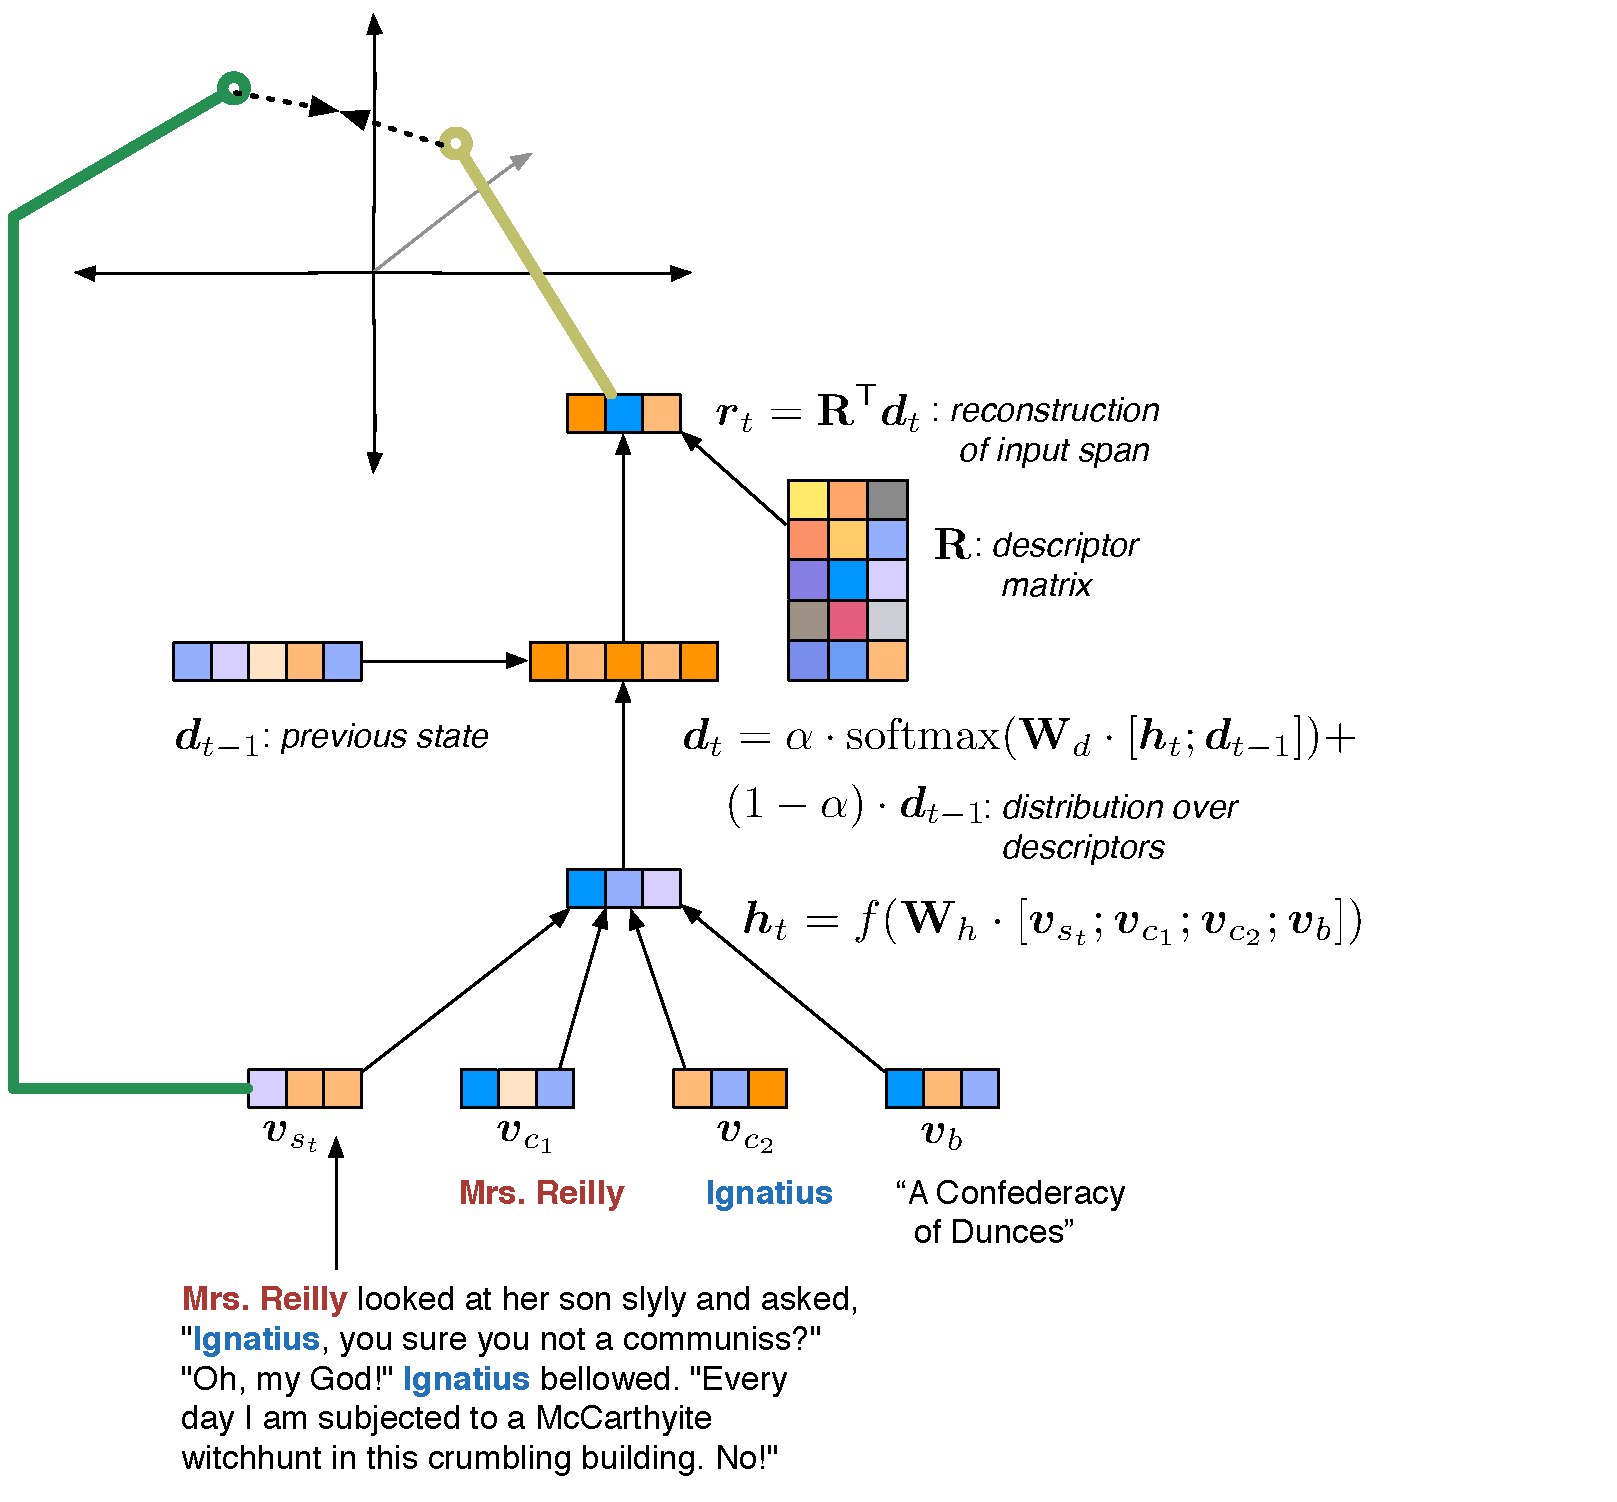
\includegraphics[width=1.15\linewidth]{2016_naacl_relationships/figures/rmn.pdf}
\caption{An example of the \rmn's computations at a single time step. The model
  approximates the vector average of an input span ($\bvec{v}_{s_t}$) as a
  linear combination of descriptors from \bmat{R}. The descriptor weights
  $\bvec{d}_t$ define the relationship state at each time step and---when viewed
  as a sequence---form a relationship trajectory.}
\label{fig:rmn}
\end{figure}

This section mathematically describes how we apply the \rmn\ to relationship
modeling on our dataset. Our model is similar in spirit to topic models: for an
input dataset, the output of the \rmn\ is a set of relationship descriptors
(topics) and---for each relationship in the dataset---a trajectory, or a
sequence of probability distributions over these descriptors (document-topic
assignments). However, the \rmn\ uses recent advances in deep learning to
achieve better control over descriptor coherence and trajectory smoothness
(Section~\ref{sec:experiments}).

\subsection{Formalizing the Problem}

Assume we have two characters $c_1$ and $c_2$ in book~$b$. We define
$S_{c_1, c_2}$ as a sequence of token spans where each span $s_t \in
S_{c_1, c_2}$ is itself a set of tokens $\{w_1, w_2, \dots, w_l\}$ of
fixed size~$l$ that contains mentions (either directly or by
coreference) to both $c_1$ and $c_2$. In other words, $S_{c_1, c_2}$
includes the text of every scene, chronologically ordered, in which
$c_1$ and $c_2$ are present together.

\subsection{Model Description}

As in other neural network models for natural language processing, we
begin by associating each word type \emph{w} in our vocabulary with a
real-valued embedding $\bvec{v}_w \in \mathbbm{R}^d$. These embeddings
are rows of a $V \times d$ matrix \bmat{L}, where $V$ is the
vocabulary size. Similarly, characters and books have their own
embeddings in rows of matrices \bmat{C} and \bmat{B}. We want
\bmat{B} to capture global context information (e.g., ``Moby Dick''
takes place at sea) and \bmat{C} to capture immutable aspects of
characters not related to their relationships (e.g., Javert is a
police officer). Finally, the \rmn\ learns embeddings for
relationship descriptors, which requires a second matrix \bmat{R} of
size $K \times d$ where $K$ is the number
of descriptors, analogous to the number of topics in topic models.

Each input to the \rmn\ is a tuple that contains identifiers for a book and two
characters, as well as the spans corresponding to their relationship: $(b, c_1,
c_2, S_{c_1,c_2})$. Given one such input, our objective is to reconstruct
$S_{c_1,c_2}$ using a linear combination of relationship descriptors from
\bmat{R} as shown in Figure~\ref{fig:rmn}; we now describe this process
formally.

\subsubsection{Modeling Spans with Vector Averages}

We compute a vector representation for each span $s_t$ in $S_{c_1,c_2}$ by
averaging the embeddings of the words in that span,
\begin{equation}\label{eq:ave}
\bvec{v}_{s_t} = \frac 1 {l} {\sum_{w \in s_t} \bvec{v}_w}.
\end{equation}
Then, we concatenate $\bvec{v}_{s_t}$ with the character
embeddings~$\bvec{v}_{c_1}$ and $\bvec{v}_{c_2}$ as well as the book embedding
$\bvec{v}_b$ and feed the resulting vector into a standard feed-forward layer to
obtain a hidden state~$\bvec{h}_t$,
\begin{equation}\label{eq:dan}
	\bvec{h}_t = f(\bmat{W}_h\cdot [\bvec{v}_{s_t};\bvec{v}_{c_1};\bvec{v}_{c_2};\bvec{v}_{b}]).
\end{equation}
In all experiments, the transformation matrix $W_h$ is
$d \times 4d$, and we set $f$ to the $\mbox{ReLu}$ function,
$\mbox{ReLu}(x) = \mathrm{max}(0, x)$.

\subsubsection{Approximating Spans with Relationship Descriptors}

Now that we can obtain representations of spans, we move on to
learning descriptors using a variant of dictionary
learning~\cite{olshausen1997sparse,elad2006image}, where our descriptor matrix \bmat{R}
is the dictionary and we are trying to approximate input spans as a
linear combination of items from this dictionary.













Suppose we compute a hidden state for every span $s_t$ in $S_{c_1,c_2}$
(Equation~\ref{eq:dan}). Now, given an $\bvec{h}_t$, we compute a weight vector
$\bvec{d}_t$ over $K$ relationship descriptors with some composition function
$g$, which is fully specified in the next section. Conceptually, each
$\bvec{d}_t$ is a \emph{relationship state}, and a \emph{relationship
  trajectory} is a sequence of chronologically-ordered relationship states as
shown in Figure~\ref{fig:traj}. After computing $\bvec{d}_t$, we use it to
compute a reconstruction vector~$\bvec{r}_t$ by taking a weighted average over
relationship descriptors,
\begin{equation}\label{eq:recon}
	\bvec{r}_t = \bmat{R}^\mathsf{T} \bvec{d}_t.
\end{equation}
Our goal is to make $\bvec{r}_t$ similar to $\bvec{v}_{s_t}$. We use a
contrastive max-margin objective function similar to previous
work~\cite{weston2011wsabie,sochergrounded}. We randomly sample spans from our
dataset and compute the vector average $\bvec{v}_{s_n}$ for each sampled span as
in Equation~\ref{eq:ave}. This subset of span vectors is $N$. The unregularized
objective~$J$ is a hinge loss that minimizes the inner product between
$\bvec{r}_t$ and the negative samples while simultaneously maximizing the inner
product between $\bvec{r}_t$ and $\bvec{v}_{s_t}$,
\begin{equation}\label{eqn:obj}
J(\theta) = \sum\limits_{t=0}^{\norm{S_{c_1,c_2}}}\sum\limits_{n \in
  N} \mathrm{max}(0, 1 - \bvec{r}_t\bvec{v}_{s_t} +
\bvec{r}_t\bvec{v}_{s_n}),
\end{equation}
where $\theta$ represents the model parameters.

\subsubsection{Computing Weights over Descriptors}

What function should we choose for our composition function~$g$ to represent a
relationship state at a given time step?  On the face of it, this seems trivial;
we can project $h_t$ to $K$ dimensions and then apply a softmax or some other
nonlinearity that yields non-negative weights.\footnote{We experiment with a
  variety of nonlinearities but find that the softmax yields the most
  interpretable results due to its predisposition to select a single
  descriptor.} However, this method ignores the relationship states at previous
time steps. To model the temporal aspect of relationships, we can add a
recurrent connection,
\begin{equation}\label{eq:rnn}
	\bvec{d}_t = \mbox{softmax}(\bmat{W}_d\cdot [\bvec{h}_t;\bvec{d}_{t-1}])
\end{equation}
where $\bmat{W}_d$ is of size $K\times (d+K)$ and
$\mbox{softmax}(\bvec{q}) = \nicefrac{\exp{\bvec{q}}}{\sum_{j=1}^k
  \exp{\bvec{q}_j}}$.

Our hope is that this recurrent connection will carry some of the previous
relationship state over to the current time step. It should be unlikely for two
characters in love at time $t$ to fall out of love at time $t+1$ even if
$s_{t+1}$ does not include any love-related words.  However, because the
objective function in Equation~\ref{eqn:obj} maximizes similarity with the
current time step's input, the model is not forced to learn a smooth
interpolation between the previous state and the current one. A natural remedy
is to have the model predict the \emph{next} time step's input instead, but this
proves hard to optimize.













We instead \emph{force} the model to use the previous relationship state by
modifying Equation~\ref{eq:rnn} to include a linear interpolation
between $\bvec{d}_{t}$ and $\bvec{d}_{t-1}$,
\begin{equation}\label{eq:rmn}
\begin{split}
	\bvec{d}_t &= \alpha \cdot \text{softmax}(\bmat{W}_d\cdot [\bvec{h}_t;\bvec{d}_{t-1}]) + \\&(1-\alpha)\cdot \bvec{d}_{t-1}.
\end{split}
\end{equation}
Here, $\alpha$ is a scalar between $0$ and $1$. We experiment with
setting $\alpha$ to a fixed value of $0.5$ as well as allowing the
model to learn $\alpha$ as in
\begin{equation}\label{eq:alpha}
	\alpha = \sigma(\bvec{v}_\alpha^\mathsf{T} \cdot[\bvec{h}_t;\bvec{d}_{t-1};\bvec{v}_{s_t}]),
\end{equation}
where $\sigma$ is the sigmoid function and $\bvec{v}_\alpha$ is a vector of
dimensionality $2d+K$.  Fixing $\alpha=0.5$ initially and then tuning it after
other parameters have converged improves training stability; for the specific
hyperparameters we use see Section~\ref{sec:experiments}.\footnote{This strategy
  is reminiscent of alternative minimization strategies for dictionary
  learning~\cite{agarwallearning}, where the dictionary and weights are learned
  separately by keeping the other fixed.}

\subsubsection{Interpreting Descriptors and Enforcing Uniqueness}
Recall that each descriptor is a $d$-dimensional row of
\bmat{R}. Because our objective function $J$ forces these descriptors
to be in the same vector space as that of the word embeddings \bmat{L}, we can
interpret them by looking at nearest neighbors in \bmat{L} using
cosine distance as the similarity metric.

To discourage learning descriptors that are too similar to
each other, we add another penalty term $X$ to our objective function,
\begin{equation}\label{eq:unique}
	X(\theta) = \euclidean{\bmat{R}\bmat{R}^\mathsf{T} - \bmat{I}},
\end{equation}
where \bmat{I} is the identity matrix. This term comes from
the component orthogonality constraint in independent component
analysis~\cite{hyvarinen2000independent}.

We add $J$ and $X$ together to obtain our final training objective $L$,
\begin{equation}\label{eq:final}
	L(\theta) = J(\theta) + \lambda X(\theta),
\end{equation}
where $\lambda$ is a hyperparameter that controls the magnitude of the
uniqueness penalty.

\section{Evaluating Descriptors and Trajectories}
\label{sec:experiments}

Because no previous work explores the interpretability of
unsupervised relationship modeling over time, evaluating the \rmn\ is
tricky. Further compounding the problem is the subjective nature of
the task; for example, is a trajectory that ignores a key event better
than one that hallucinates episodes absent from source text?

With these issues in mind, we conduct three evaluations to show that our output
is reasonable. First, we conduct a crowdsourced interpretability experiment that
shows \rmn s produce significantly more coherent descriptors than three topic
model baselines. A second crowdsourced task indicates that our model produces
trajectories that match plot summaries more accurately than topic
models. Finally, we qualitatively compare the \rmn's output to existing static
annotations of literary relationships and find both expected and surprising
results.

\subsection{Topic Model Baselines}

Before moving onto the evaluations, we briefly describe three baseline models,
all of which are Bayesian generative models. Latent Dirichlet
allocation~\cite[\lda{}]{blei2003latent} learns a single document-topic
distribution per document; we can apply \lda\ to our dataset by concatenating
all spans from a relationship into a single document. Similarly,
\nubbi~\cite{chang2009connections} learns separate sets of topics for
relationships and individual characters.\footnote{\nubbi\ requires additional
  spans that mention only a single character to differentiate character topics
  from relationship topics. None of the other models receives these extra data.}

\lda\ and \nubbi\ are incapable of taking into account the chronological
ordering of the spans because they view all relationships tokens as
exchangeable. While we can compare the \emph{descriptors} learned by these
models to those of the \rmn, we cannot evaluate their \emph{trajectories}. We
turn instead to the hidden topic Markov model~\cite[\htmm]{gruber2007hidden},
which foregoes the bag-of-words assumption of \lda\ and \nubbi\ in favor of
modeling topic segments within a document as a Markov chain. This model outputs
a smooth sequence of topic assignments over a document, so we can compare the
\emph{trajectories} it learns on our dataset to those of the \rmn.

\subsection{Experimental Settings}

In our descriptor interpretability experiments, we vary the number of
descriptors (topics) for all models ($K=10,30,50$). We train \lda\ and
\nubbi\ for 100 iterations with a collapsed Gibbs sampler, and the \htmm\ uses
the default setting of 100 \abr{em} iterations.










For the \rmn, we initialize the word embedding matrix \bmat{L} with
300-dimensional GloVe embeddings trained on the Common
Crawl~\cite{glove2014}. The character and book embeddings (\bmat{C} and
\bmat{B}) are initialized randomly. We fix $\alpha$ to 0.5 for the first 15
epochs of training; after the descriptor matrix \bmat{R}\ has converged, we fix
\bmat{R}\ and tune $\alpha$ using Equation~\ref{eq:rmn} for 15 more
epochs.\footnote{Preliminary experiments show that learning $\alpha$ and
  \bmat{R} simultaneously results in less interpretable descriptors.} Since the
topic model baselines do not have access to character and book metadata, for
fair comparison we also train a ``generic'' version of the \rmn\ (\grmn) where
the metadata embeddings are removed from Equation~\ref{eq:dan}. The uniqueness
penalty $\lambda$ is set to $10^{-4}$.








All of the \rmn\ model parameters except \bmat{L} are optimized using
Adam~\cite{kingma2014adam} with a learning rate of 0.001 for 30 epochs; the word
embeddings are not fine-tuned during training.\footnote{Tuning \bmat{L} ruins
  descriptor interpretability; pretrained embeddings are likely already a good
  solution for our problem.} We also apply word dropout~\cite{IyyerDAN} to the
input spans, removing words from the vector average computation in
Equation~\ref{eq:ave} with probability 0.5.

\begin{table*}[ht]
\centering
\begin{tabular}{llp{5cm}llp{5cm}}
\toprule
\multicolumn{3}{c}{\bf RMN} & \multicolumn{3}{c}{\bf HTMM} \\
\cmidrule(l{10pt}r{10pt}){1-3}
\cmidrule(l{10pt}r{10pt}){4-6}
\bf Label & \bf MP & \bf Nearest Neighbors & \bf Label & \bf MP & \bf Most Probable Words \\
\midrule
sadness & 1.0 & \footnotesize regretful rueful pity pained despondent & violence & 1.0 & \footnotesize sword shot blood shouted swung \\
love & 1.0 & \footnotesize love delightful happiness enjoyed & boats & 1.0 & \footnotesize ship boat captain deck crew \\
murder & 1.0 & \footnotesize autopsy arrested homicide murdered & food & 1.0 & \footnotesize kitchen mouth glass food bread \\
\midrule
worship & 0.1 & \footnotesize toil pray devote yourselves gather & sci-fi & 0.0 & \footnotesize suppose earth robots computer certain \\
moodiness & 0.3 & \footnotesize glumly snickered quizzically guiltily & fantasy & 0.0 & \footnotesize agreed magician dragon castle talent\\
informal & 0.4 & \footnotesize kinda damn heck guess shitty& military & 0.1 & \footnotesize ship captain lucky hour general \\
\bottomrule
\end{tabular}

\caption{Three high-precision (top) and three low-precision (bottom) descriptors for the \rmn\ and \htmm, along with labels from an external evaluator and model precision (\abr{mp}) computed via word intrusion experiments. The \rmn\ is able to learn a variety of interpersonal states (e.g., \underline{love}, \underline{sadness}), while the \htmm's most coherent topics are about concrete objects or events.}
\label{table:intrusion}
\end{table*}

\subsection{Do Descriptors Make Sense?}

\begin{figure}[t!]
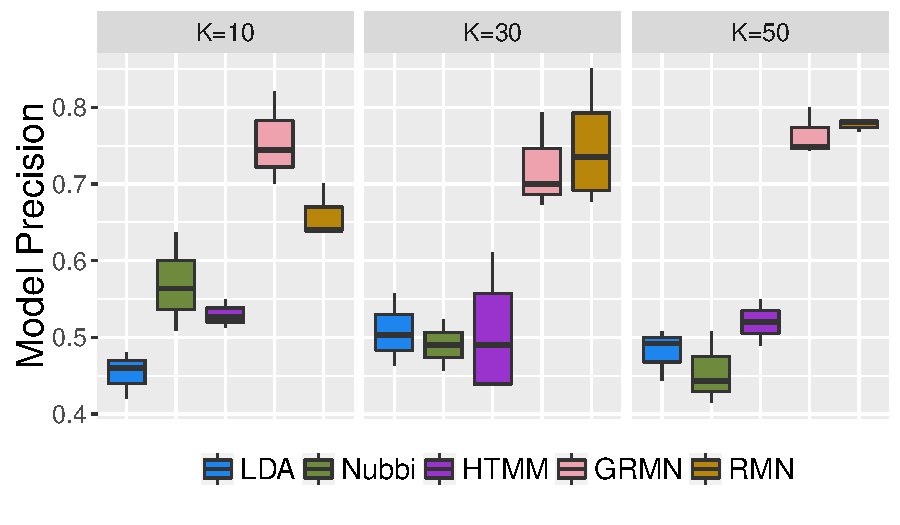
\includegraphics[width=1.0\linewidth]{2016_naacl_relationships/figures/topic_intrusion.pdf}
  \caption{Model precision results from our word intrusion task. The \rmn\
  learns more interpretable descriptors than three topic model baselines.}
\label{fig:intrusion}
\end{figure}

The goal of our first experiment is to compare the descriptors
\bmat{R} learned by the \rmn\ to the topics learned by the topic model
baselines. We conduct a word intrusion
experiment~\cite{chang2009reading}: workers identify an ``intruder''
word from a set of words that---other than the intruder---come from
the same topic. For the topic models, the five most probable words are
joined by a highly-probable word from a different topic as the
intruder. We use the same procedure for the \rmn\ and \grmn, except that
cosine similarity to descriptor embeddings replaces topic-word
probability. To control for randomness in the training process, we
train three of each model, so the final experiment consists of 1,350
tasks ($K=10,30,50$ descriptors per trial, three trials per model).

We collect judgments from ten different workers for each task using the
Crowdflower platform.\footnote{\url{http://www.crowdflower.com}} Our evaluation
metric, model precision (\abr{mp}), is the fraction of workers that select the
correct intruder word for a descriptor $k$.  Low model precision signals
descriptors that lack cohesive themes.

On average, the \rmn's descriptors are much more interpretable than those of the
baselines, as it achieves a mean model precision of 0.73
(Figure~\ref{fig:intrusion}) across all values of $K$.  There is little
difference between the model precision of the three topic model baselines,
which hover around 0.5. There is also little difference between the \grmn\ and
\rmn; however, visualizing the learned character and book embeddings as in
Figure~\ref{fig:bookpca} may be insightful for literary scholars. We show
example high and low precision descriptors for the \rmn\ and \htmm\ in
Table~\ref{table:intrusion}; a full list is included in the supplementary
material.

\subsection{Do Trajectories Make Sense?}

While the previous evaluation focused only on descriptor quality, our next
experiment compares the trajectories learned by the best \rmn\ model from the
intrusion experiment (measured by highest mean model precision) to those learned
by the best \htmm\ model, which is the only baseline capable of learning
relationship trajectories. Workers read a plot summary and choose which model's
trajectory best represents the relationship in question. We use the $K=30$
setting because it provides the best balance between descriptor variety and
trajectory interpretability.

For this evaluation, we crawl Wikipedia, Goodreads, and SparkNotes for plot
summaries associated with our 1,383 books. We then remove all relationships
where each involved character is not mentioned at least five times in the
summary, which results in a final evaluation set of 125
relationships.\footnote{Without this filtering step, workers do not have enough
  information to compare the two models since most of the characters in our
  dataset are not mentioned in summaries.}  We present workers with two
characters, a plot summary, and a visualization of trajectories learned by the
\rmn\ and the \htmm\ (Figure~\ref{fig:cftask}). The workers then select the
trajectory that best matches the relationship described by the summary.

To generate the visualizations, we first have an external annotator label each
descriptor from both models with a single word as in
Table~\ref{table:intrusion}. For fairness, the annotator is unaware of the
underlying models. For the \rmn, we visualize trajectories by displaying the
label of the argmax over descriptor weights $\bvec{d}_t$ at each time step
$t$. Similarly, for the \htmm, we display the most probable topic at each time
step.\footnote{To reduce visual clutter, we ignore descriptors that persist for
  only a single time step.}

The results of this task with seven workers per comparison favor the \rmn: for
87 out of the 125 evaluated relationships (69.6\%), the workers choose the
\rmn's trajectory over the \htmm's. We compute the Fleiss $\kappa$
value~\cite{fleiss1971measuring} to correct our inter-annotator agreement for
chance and find that $\kappa = 0.32$, indicating fair agreement among the
workers. Furthermore, thirty-four relationships had unanimous agreement among the seven
workers; of these, twenty-six were unanimous in favor of the \rmn\ compared to only eight
for the \htmm.

\begin{figure}[t!]
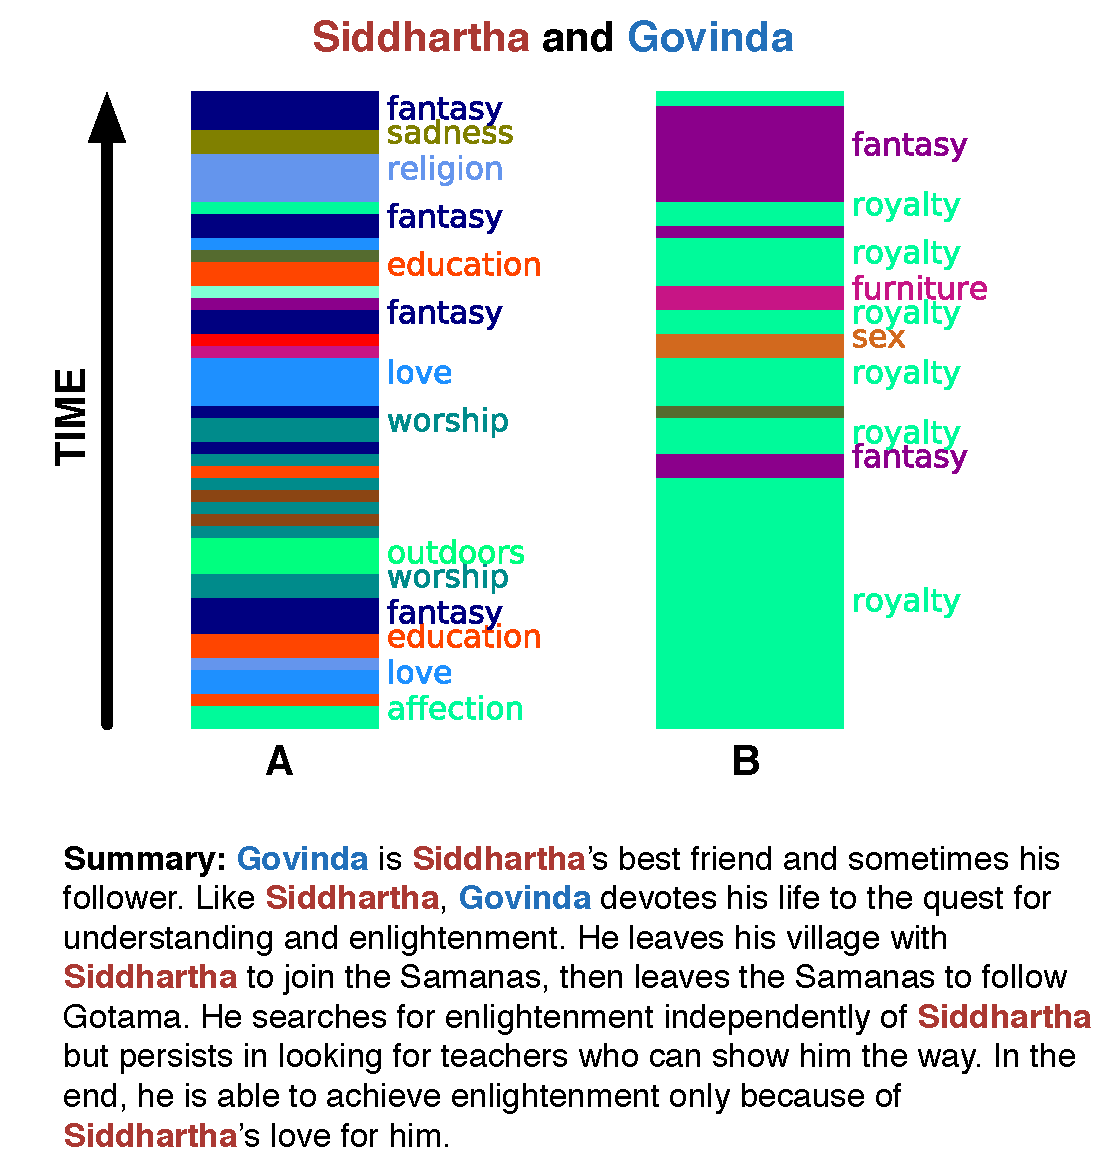
\includegraphics[width=1.0\linewidth]{2016_naacl_relationships/figures/cftask.pdf}
  \caption{An example from the Crowdflower summary matching task;
    workers are asked to choose the trajectory (here, ``A'' is generated by the
    \rmn\ and ``B'' by the \htmm) that best matches a provided summary that
    describes the relationship between Siddartha and Govinda (from
    \textit{Siddartha} by Hesse).}
\label{fig:cftask}
\end{figure}

\subsection{What Makes a Relationship Positive?}

While the previous two experiments show that the \rmn\ is more interpretable and
accurate than baseline models, we have not yet shown that its insights can aid
in drawing connections across various books and genres. As a first step in this
direction, we investigate what makes a relationship positive or negative by
comparing trajectories from the \rmn\ and \htmm\ to static affinity annotations
from a recently-released dataset~\cite{massey2015annotating} of fictional
relationships. Expected correlations (e.g., \underline{murder} and
\underline{sadness} are strongly negative descriptors) emerge alongside
surprising ones (\underline{politics} is negative, \underline{religion} is
positive).

The affinity labeling task of \newcite{massey2015annotating} requires workers to describe a given
relationship as positive, negative, or neutral. We consider only
non-neutral relationships for which two annotators agree on the affinity label and
remove all books not present in our own dataset. This filtering step results in 120
relationships, 78\% of which are positive and the remaining 22\% negative.

Since the annotations are static, we first aggregate our trajectories
across all time steps. We compute $K$-dimensional ``average positive'' and
``average negative'' weight vectors $\bvec{a}_p$ and $\bvec{a}_n$ by averaging
the relationship states $\bvec{d}_t$ for the \rmn\ and the document-topic
distributions for the \htmm\ across all time steps for relationships labeled
with a particular affinity. Then, we compute the vector difference $\bvec{a}_p -
\bvec{a}_n$ and sort it to produce a ranked list of descriptors, where
descriptors with positive differences occur more frequently in positive
relationships. Table~\ref{table:affinity} shows the most positive and most
negative descriptors; of particular interest is the large negative weight associated with political relationships from both models.

\begin{table}[t!]
\centering
\begin{tabular}{lp{2.8cm}p{2.8cm}}
\toprule
\bf Model & \bf Positive & \bf Negative\\
\midrule
\rmn & \footnotesize education, \textcolor{blue}{love}, religion, \textcolor{blue}{sex} & \footnotesize politics, \textcolor{red}{murder}, \textcolor{red}{sadness}, royalty \\
\htmm & \footnotesize \textcolor{blue}{love}, \textcolor{blue}{parental}, business, outdoors & \footnotesize \textcolor{blue}{love}, politics, \textcolor{red}{violence}, \textcolor{red}{crime} \\
\bottomrule
\end{tabular}

\caption{Descriptors most characteristic of positive and negative relationships,
  computed using existing annotations. Compared to the \rmn, the
  \htmm\ struggles to coherently characterize negative relationships. Interestingly, both models show negative predispositions for political
  relationships, perhaps due to genre bias or class differences. }

\label{table:affinity}
\end{table}

\section{Qualitative Analysis}
\label{sec:discussion}

\begin{figure*}[ht]
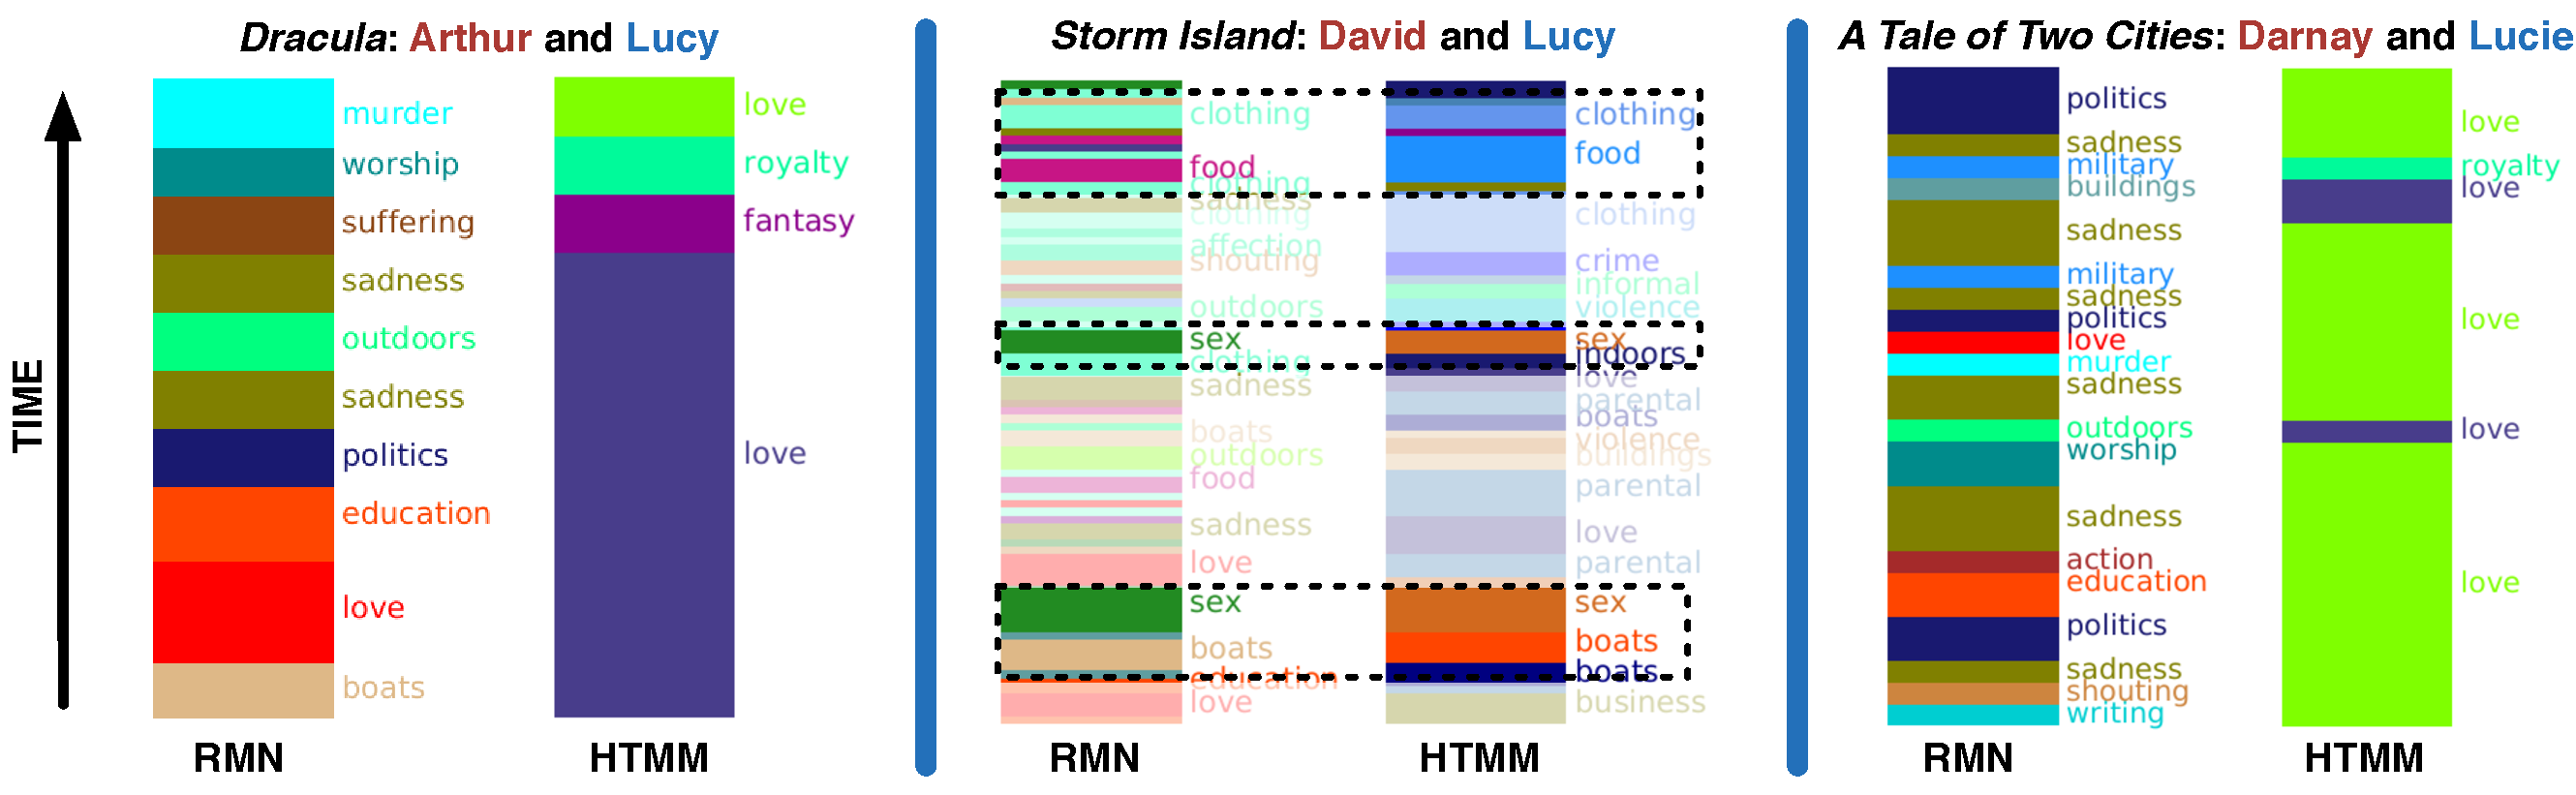
\includegraphics[width=1.0\linewidth]{2016_naacl_relationships/figures/good_bad_traj.pdf}
  \caption{\emph{Left}: the \rmn\ is able to model Arthur and Lucy's trajectory
    reasonably well compared to our manually-created version in
    Figure~\ref{fig:traj}. \emph{Middle}: both models agree on event-based
    descriptors such as \underline{food} and \underline{sex}. \emph{Right}: a
    failure case for the \rmn\ in which it is unable to learn that Lucie Manette
    and Charles Darnay are in love.}
\label{fig:goodbadtraj}
\end{figure*}

\begin{figure*}[ht]
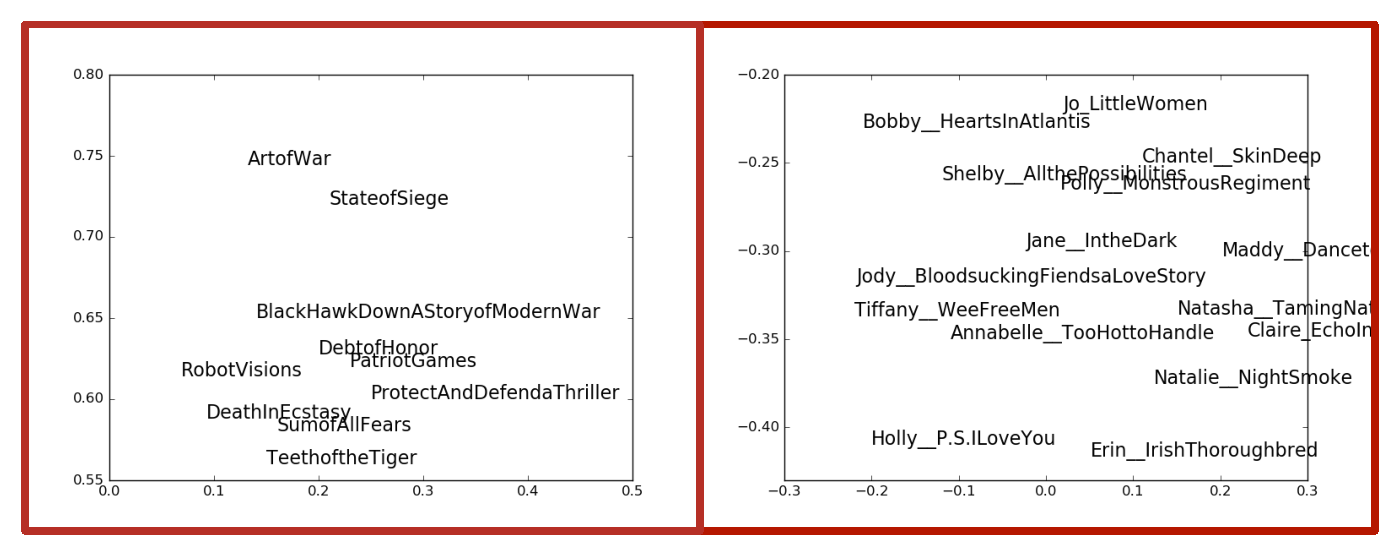
\includegraphics[width=1.0\linewidth]{2016_naacl_relationships/figures/charbookembeddings.pdf}
  \caption{Clusters from \abr{pca} visualizations of the \rmn's learned book (left) and character (right) embeddings. We see a cluster of books about war and violence (many of which are authored by Tom Clancy) as well as a cluster of lead female characters from primarily romance novels. These visualizations show that the \rmn\ can recover useful static representations of characters and books in addition to the dynamic relationship trajectories.}
\label{fig:bookpca}
\end{figure*}

Our experiments show the superiority of the \rmn\ over various topic model
baselines in both descriptor interpretability and trajectory accuracy, but what
causes the improved performance? In this section, we analyze similarities
between the \rmn\ and \htmm\ and look at qualitative examples where the
\rmn\ succeeds and fails. We also connect the findings of our affinity
experiment to existing literary scholarship.

Both models are equally proficient at learning and assigning event-based
descriptors (e.g., \underline{crime}, \underline{violence},
\underline{food}). More specifically, the \rmn\ and \htmm\ agree on
environmental descriptions (e.g., boats, outdoors) and graphic sexual scenes
(Figure~\ref{fig:goodbadtraj}, middle).

However, the \rmn\ is more sophisticated with interpersonal relationships. None
of the topic model baselines learns negative emotional descriptors such as
\underline{sadness} or \underline{suffering}, which explains the inaccurate
\htmm\ trajectory of Arthur and Lucy in the left-most panel of
Figure~\ref{fig:goodbadtraj}. All of the topic model baselines learn
duplicate topics; in Table~\ref{table:affinity}, one \underline{love} descriptor
is highly positive while a duplicate is strongly negative.\footnote{This
  ``duplicate love'' phenomenon persists even when we reduce the number of
  topics.} The \rmn\ circumvents this problem with its uniqueness penalty
(Equation~\ref{eq:unique}).

While the increased descriptor variety is a positive, sometimes it leads the
\rmn\ astray. The model largely ignores the love between Charles Darnay and
Lucie Manette in Dickens' \emph{A Tale of Two Cities} due to book's sad tone;
meanwhile, the \htmm's trajectory, while vastly simplified, does pick up on the
romance (Figure~\ref{fig:goodbadtraj}, right). While the \rmn's learnable book
and character embeddings should help, the signal in a span cannot lead to the
``proper'' descriptor.

Both the \rmn\ and \htmm\ learn that \underline{politics} is strongly negative
(Table~\ref{table:affinity}). Existing scholarship supports this finding:
Victorian-era authors, for example, are ``obsessed with \emph{otherness} \dots of
antiquated social and legal institutions, and of autocratic and/or dictatorial
abusive government''~\cite{zarifopol1995kill}, while in science fiction,
``dystopia—--precisely because it is so much more common (than utopia)—--bears
the aspect of lived experience''~\cite{gordin2010utopia}. Our affinity data
comes primarily from Victorian novels (e.g., by Dickens and George Eliot),
leading us to believe that that the models are behaving reasonably. Finally,
returning to the ``extra'' meaning of meals discussed in
Section~\ref{sec:introduction}, \underline{food} occurs
\emph{slightly} more frequently in positive relationships.

\section{Related Work}
\label{sec:related}

There are two major areas upon which our work builds: computational literary
analysis and deep neural networks for natural language processing.

Most previous work in computational literary analysis has focused either on
characters or events. In the former category, graphical models and classifiers
have been proposed for learning character personas from
novels~\cite{bamman-underwood-smith:2014:P14-1,flekova2015personality} and film
summaries~\cite{bamman-oconnor-smith:2013:ACL2013}. The \nubbi\ model of
\newcite{chang2009connections} learns topics that statically describe characters
and their relationships. Because these models lack temporal components (the
focus of our task), we compare instead against the
\htmm\ of \newcite{gruber2007hidden}.

Closest to our own work is the supervised structured
prediction problem of \newcite{snigdhachars}, in which features are
designed to predict dynamic sequences of positive and negative
interactions between two characters in plot summaries. Other research in this area
includes social network construction from
novels~\cite{elson2010extracting,Srivastava:2016} and film~\cite{krishnan2015youre},
as well as attempts to summarize and generate
stories~\cite{elsner2012character}. 

While some of the relationship descriptors learned by our model are
character-centric, others are more events-based, depicting actions rather than
feelings; such descriptors have been the focus of much previous
work~\cite{schankabelson77,chambers2008unsupervised,chambers2009unsupervised,orr2014learning}. Our
model is more closely related to the plot units
framework~\cite{lehnert1981plot,daume13plotunits}, which annotates events with
emotional states.

The \rmn\ builds on deep recurrent autoencoders such as the hierarchical
\abr{lstm} autoencoder of \newcite{li2015hierarchical}; however, it is more
efficient because of the span-level vector averaging. It is also similar to
recent neural topic model architectures~\cite{cao2015novel,dasacl2015}, although
these models are limited to static document representations. We hope to apply the \rmn\ to nonfictional datasets as well; in this vein, \newcite{IyyerEtAl2014} apply a neural network to sentences from nonfiction political books for ideology prediction.

More generally, topic models and related generative models are a central tool
for understanding large corpora from science~\cite{talley-11} to
politics~\cite{Nguyen-14b}. We show representation learning models
like \rmn\ can be just as interpretable as \abr{lda}-based models. Other
applications for which researchers have prioritized interpretable vector
representations include text-to-vision mappings~\cite{lazaridou2014wampimuk} and
word embeddings~\cite{fyshe2015compositional,faruqui2015sparse}.

\section{Conclusion}
\label{sec:conclusion}

We formalize the task of unsupervised relationship modeling, which
involves learning a set of relationship descriptors as well as a trajectory over
these descriptors for each relationship in an input dataset. We present the
\rmn, a novel neural network architecture for this task that generates more
interpretable descriptors and trajectories than topic model baselines. Finally,
we show that the output of our model can lead to interesting insights when
combined with annotations in an existing dataset.


\section*{Acknowledgments}

We thank Jonathan Chang and Amit Gruber for providing baseline code, Thang Nguyen for helpful discussions about our model, and the anonymous reviewers for their insightful comments.
This work was supported by \abr{nsf} grant \abr{iis}-1320538.
Boyd-Graber is also partially supported by \abr{nsf} grants
\abr{ccf}-1409287 and \abr{ncse}-1422492. Any opinions, findings,
conclusions, or recommendations expressed here are those of the
authors and do not necessarily reflect the view of the sponsor.

\clearpage

\bibliographystyle{style/naaclhlt2016}
\bibliography{bib/journal-full,bib/miyyer,bib/jbg}


\end{document}
